\documentclass[tikz,border=2pt]{standalone}
\usepackage{pgfplots}
\pgfplotsset{compat=1.18}
\usetikzlibrary{positioning}
\usepackage{helvet}
\renewcommand{\familydefault}{\sfdefault}
\definecolor{ieeecolor}{HTML}{042C53}
\definecolor{jrnlcolor}{HTML}{378ADD}
\definecolor{othercolor}{HTML}{B4B2A9}
\definecolor{confcolor}{HTML}{D98B3F}
\begin{document}
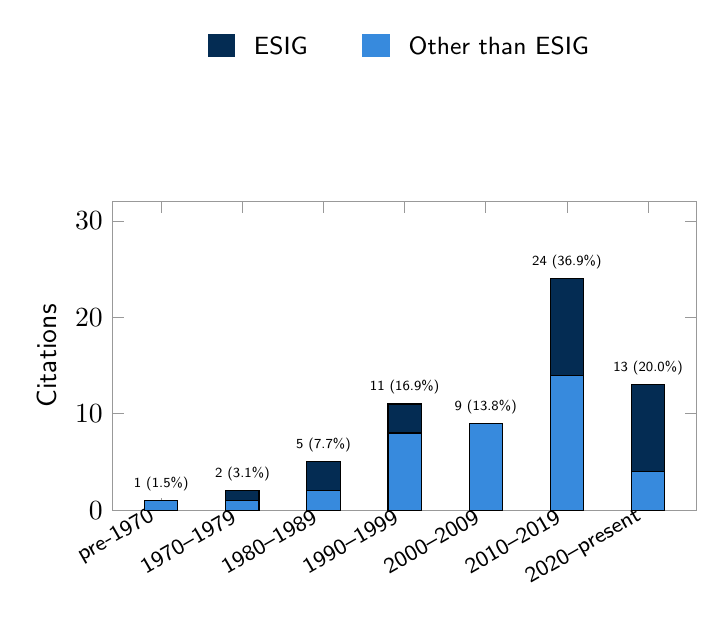
\begin{tikzpicture}
\begin{axis}[
    ybar stacked, bar width=12pt,
    width=9cm, height=5.5cm,
    symbolic x coords={pre-1970,1970--1979,1980--1989,1990--1999,2000--2009,2010--2019,2020--present},
    xtick=data,
    x tick label style={rotate=30, anchor=east, font=\footnotesize},
    ylabel={Citations},
    ymin=0, ymax=32,
    axis line style={color=black!40},
    tick style={color=black!40},
    enlarge x limits=0.1,
]
\addplot[fill=jrnlcolor] coordinates {(pre-1970,1) (1970--1979,1) (1980--1989,2) (1990--1999,8) (2000--2009,9) (2010--2019,14) (2020--present,4)};
\addplot[fill=ieeecolor] coordinates {(pre-1970,0) (1970--1979,1) (1980--1989,3) (1990--1999,3) (2000--2009,0) (2010--2019,10) (2020--present,9)};
\node[font=\tiny, anchor=south] at (axis cs:pre-1970,1) {1 (1.5\%)};
\node[font=\tiny, anchor=south] at (axis cs:1970--1979,2) {2 (3.1\%)};
\node[font=\tiny, anchor=south] at (axis cs:1980--1989,5) {5 (7.7\%)};
\node[font=\tiny, anchor=south] at (axis cs:1990--1999,11) {11 (16.9\%)};
\node[font=\tiny, anchor=south] at (axis cs:2000--2009,9) {9 (13.8\%)};
\node[font=\tiny, anchor=south] at (axis cs:2010--2019,24) {24 (36.9\%)};
\node[font=\tiny, anchor=south] at (axis cs:2020--present,13) {13 (20.0\%)};
\end{axis}
\begin{scope}[shift={(1.2,5.9)}]
\node[fill=ieeecolor, minimum width=10pt, minimum height=8pt, anchor=west] (legbox0) at (0,0) {}; \node[anchor=west, font=\small, right=3pt of legbox0] (legtxt0) {ESIG}; \node[fill=jrnlcolor, minimum width=10pt, minimum height=8pt, anchor=west, right=16pt of legtxt0] (legbox1) {}; \node[anchor=west, font=\small, right=3pt of legbox1] (legtxt1) {Other than ESIG};
\end{scope}
\end{tikzpicture}
\end{document}
